\chapter{Analyse af anvendelsesområdet}
\label{chap:analyseafao}

I følgende kapitel analyseres anvendelsesområdet, som er de organisationsdele, der administrerer, overvåger og styrer problemområdet. Analysen tager udgangspunkt i en metode, som er introduceret i bogen \emph{Objekt Orienteret Analyse og Design} \cite[p. ~113]{ooad}. 

Formålet med analysen af anvendelsesområdet, er at fastsætte kravene til brugen af systemet. Dette gøres ved først at undersøge, hvilke aktører, der interagerer med systemet, og til sidst fastlægge hvilke funktioner, der skal være tilgængelig for aktørerne. Målet opnås ved at udarbejde brugsmønstre og samarbejde med eventuelle brugere, som vores informanter, for at finde ud af, hvordan systemet kan blive brugt.

I \secref{sec:brug} identificerer vi først hvilke aktører, der findes, og derefter hvordan disse aktører kan bruge systemet, ved at udarbejde brugsmønstre.

% Anvendelsesområde
\section{Brug}
\label{sec:brug}
Denne analyse af anvendelsesområdets brug, har til formål at gøre det klart, hvilke aktører, der benytter \Foodl{}. Resultatet af analysen af aktører er en mængde aktørbeskrivelser. Resultatet af denne akvitet er brugsmønstre. Hver enkelt brugsmønster vedrører en eller flere aktører. Denne relation vises i \tableref{table:aktoertabel}. Et flueben betyder at brugsmønstret i samme række vedrører aktøren i samme kolonne.

\begin{table}
  \centering
    \begin{tabular}{ r|c c c }
  \hline
                       &    \multicolumn{3}{c}{\textbf{Brugsmønstre}}   \\ 
\textbf{Aktører}       & Bruger     & Administrator & Crawler    \\ \hline 
Søgning                & \checkmark &               &            \\ 
Favorisering           & \checkmark &               &            \\ 
Indkøbslistehåndtering & \checkmark &               &            \\ 
Login                  & \checkmark & \checkmark    &            \\ 
Fejlhåndtering         &            & \checkmark    &            \\ 
Rapportering           & \checkmark & \checkmark    &            \\ 
Crawling               &            &               & \checkmark \\
    \hline
    \end{tabular}
    \capt{Aktørtabel for Foodl.}
    \label{table:aktoertabel}
\end{table}


\subsection{Aktører}
\label{sec:aktoerer}
Vi har identificeret 3 aktører (Bruger, Administartor og Dataudtrækker), som også er vist i \tableref{table:aktoertabel}, der vil kunne interagere med \Foodl{}. Vi specificerer aktører med en beskrivelse af aktøren og om nødvendigt en eller flere eksempler på hver enkelt aktør.

Disse beskrivelser har til formål at give læseren en bedre forståelse for, hvilke egenskaber og karakterisitka en sådan aktør besidder. 


\aktortabelEx{Bruger}
{En person, der ønsker at bruge systemet foodl.dk til at finde opskrifter, der er mulige at lave med de råvarer, som personen er i besiddelse af.}
{Systemets brugere inkluderer mange personer i forskellige aldersgrupper med vidt forskellig erfaring inden for computerbrug.}
{Bruger A er en 23-årig universitetsstuderende, der føler sig sikker med at navigere rundt på internettet og gør det flere gange dagligt. A kan godt lide at afprøve de forskellige funktioner som hjemmesider stiller til rådighed, for at undersøge hvad de gør. A er meget lærenem, når det kommer til at benytte funktioner på hjemmesider. A bor alene, og har pga. supermarkedernes familietilpassede portioner, ofte madrester til overs, som A ønsker at bruge. Systemet bliver brugt til at få madresterne med i aftenens aftensmad. 

Bruger B er en 45-årig familiemor eller -far, der hovedsagligt bruger computeren til arbejdsrelaterede opgaver og til at holde sig opdateret ved at læse nyheder på diverse nyhedshjemmesider. Bruger B benytter systemet til blandt andet at få brugt madrester fra den foregående dags aftensmad eller til at få inspiration til den kommende aftensmad. Bruger B vil være interesseret i at være i stand til at dele f.eks. indkøbsliste med ægtefællen, på tværs af enheder.}
{}

\aktortabelEx{Administrator}{ak-administrator}
{En person, der har til formål at administrere og håndtere eventuelle fejl i systemet, der rapporteres af systemets brugere.}
{Systemets administrator har et højt erfaringsniveau med hensyn til systemet. De har også kontakt til systemets udviklere, der kan rette eventuelle seriøse og systemkritiske fejl.}
{Administrator A er en ubetalt studerende, som håndterer fejl på \Foodl{} i sin fritid. A gennemgår fejlrapporter og vurderer om en fejl er så kritisk at han bør kontakte en systemudvikler, eller om han selv kan udbedre fejlen, \fx ved at slette et dødt link.}
{}


  \begin{tabular}{p{\textwidth}}
    \hline
    \begin{center} \textbf{\textit{Crawler}} \end{center} \\ \hline
    \textbf{Formål:} Et system, der skal besøge foruddefinerede hjemmesider indeholdende opskrifter, som crawleren skal analysere, oversætte og gemme oplysningerne i en database. \\ 
    \textbf{Karakteristik:} Crawleren fungerer systematisk ud fra nogle foruddefinerede parametre. Der findes én crawler til hver opskriftshjemmeside, fordi hjemmesiderne ikke nødvendigvis er opbygget på samme måde. Dette betyder, at de samme parametre ikke nødvendigvis vil gælde for flere opskriftshjemmesider. \\ \hline
  \end{tabular}




\subsection{Brugsmønstre}
\label{subsec:brugsmoenstre}
For at beskrive hændelserne, der vedører en given aktør, modellerer vi en række brugsmønstre. Brugsmønstrene præsenteres både i form af  tilstandsdiagrammer og brugsmønsterspecifikationer. Tilstandsdiagramet giver et visuelt overblik over brugsmønsteret, hvor brugsmønsterspecifikation giver en mere detaljeret beskrivelse af brugsmønsteret.

I forbindelse med modelleringen af brugsmønstre, har vi fokuseret på, at identificere så mange brugsmønsterkandidater som muligt. Vi har benyttet denne teknik i et forsøg på at sikre, i at vi ikke har overset et vigtigt brugsmønster. Kandidaterne er valgt i forbindelse med en brainstorming, og er hver især blevet analyseret for relevans efter brainstormen. Dette har resulteret i at nogle af kandidaterne er blevet fravalgt. Der har været flere grunde til, at vi har fravalgt kandidater:

\begin{itemize}[noitemsep]
\item Brugsmønstret har ikke været en del af anvendelsesområdet
\item Brugsmønstret har været for simpelt
\item Brugsmønstret har været været en del af eller magen til et andet brugsmønstre
\end{itemize}

De fravalgte kandidater, samt begrundelsen fra fravælgelsen fremgår af \apref{ap:fravalgtebrugsmoenstre}.



\begin{table}[h]
\brugtabel{Favorisering}
{Favorisering igangsættes af brugeren. Når brugeren har lavet en søgning, og flere forskellige opskrifter vises som søgeresultater, kan brugeren klikke på favorisér-knappen tilhørende den enkelte opskrift, for at favorisere denne. Når en opskrift er blevet favoriseret, tilføjes denne til en liste af favoritopskrifter. Det er muligt at fjerne opskriften fra favoritlisten på to måder. Enten fra samme sted, som favoriseringen blev tilføjet, eller direkte i favoritlisten.}
{}
{}


%Noget er fucked up med brugsmoenstrene, der burde være konverteret. Der mangler x.pdf filerne
%\begin{figure}
%\centering
%\def \svgwidth{\columnwidth}
%\brugtabel{Favorisering}
{Favorisering igangsættes af brugeren. Når brugeren har lavet en søgning, og flere forskellige opskrifter vises som søgeresultater, kan brugeren klikke på favorisér-knappen tilhørende den enkelte opskrift, for at favorisere denne. Når en opskrift er blevet favoriseret, tilføjes denne til en liste af favoritopskrifter. Det er muligt at fjerne opskriften fra favoritlisten på to måder. Enten fra samme sted, som favoriseringen blev tilføjet, eller direkte i favoritlisten.}
{}
{}

%\end{figure}

\end{table}

\begin{table}[h]
\begin{tabular}{p{\textwidth}}
    \hline
    \begin{center} 
    \textbf{\textit{Rapportering}} 
    \end{center} \\ \hline
    \textbf{Brugsmønster:} Rapportering igangsættes af brugeren, når denne opdager en fejl på hjemmesiden. Hvis brugeren opdager en fejl, der har med et søgningsresultat (opskrift) at gøre, så klikkes der på en rapporteringsknap, der er ved det enkelte søgningsresultatet. Når der skal rapporteres en fejl vedrørende opskrifter, så åbnes en dialogboks på siden, hvor brugeren herefter skal vælge en fejltype. Der skelnes mellem beskrivelige og ubeskrivelige fejltyper. Et eksempel på en ubeskrivelig fejltype er bl.a., hvis et link ikke fungerer, som hører under fejltypen “dødt link”. De ubeskrivelige fejltyper behøver ingen beskrivelse, da fejltypen er beskrivelse nok i sig selv. Vælger brugeren derimod en beskrivelig fejltype, så præsenteres en beskrivelsesboks for brugeren, hvor fejlen beskrives med tekst. Derefter er rapporten klar, og brugeren skal nu godkende rapporten, inden den bliver sendt til administratoren.
Derudover er der en generel rapporteringsknap, der vedrører andre, generelle fejl på siden. Når denne knap benyttes, så dirigeres brugeren direkte hen til en beskrivelsesboks, hvor fejlen beskrives med tekst. Til slut skal rapporten godkendes af brugeren, inden den bliver sendt til administratoren. Det er altid muligt at annullere rapporteringen under alle tilstande i brugsmønstret. \\
    \textbf{Objekter:}  \\
    \textbf{Funktioner:}  \\ \hline
\end{tabular}
\todo{INDSÆT BILLEDE AF BRUGSMØNSTER}
\end{table}

\begin{table}[h]
\brugtabel{Fejlhåndtering}
{Fejlhåndering igangsættes af \textit{administratoren}. \textit{Administratoren} logger ind på hjemmesiden, og bevæger sig ind på fejlhåndteringssiden. Her præsenteres en liste af  fejlrapporter, der, via \textit{brugeren}, er blevet rapporteret og dokumenteret i systemet. \textit{Administratoren} kan derefter klikke på en fejlrapport i listen for at se en detaljeret beskrivelse af den givne fejl, som derefter kan håndteres.}
{}
{}

\begin{figure}
\centering
\scalebox{0.7}{
\input{billeder/brugsmoenstre/fejlhaandtering.pdf_tex}
}
\capt{Brugmønsteret fejlhåndtering}\label{fig:bm-fejlhaandtering}
\end{figure}


\todo{INDSÆT BILLEDE AF BRUGSMØNSTER}
\end{table}

\begin{table}[h]
\brugtabel{Indkøbslistehåndtering}{indkoebslistehaandtering}
{Håndteringen af indkøbslisten følger materialemønsteret\cite[p.~128]{ooad}. I materialemønstret er det muligt for aktøreren, at lave flere handlinger i en vilkårlig rækkefølge, da der i brugmønstret typisk ikke vil være særlig mange tilstande i forhold til handlinger. Håndteringen igangsættes af \textit{brugeren}. \textit{Brugeren} kan tilgå indkøbslisten fra en vilkårlig underside på \Foodl. Når \textit{brugeren} har tilgået indkøbslisten, så er redigeringen igangsat, og det er muligt at tilføje/fjerne varer fra indkøbslisten. Ingredienser bliver ``omdannet'' til varer, når de tilføjes på indkøbslisten. Alle elementer på indkøbslisten er af vare-klassen, hvilket gør det muligt for \textit{brugeren} at indtaste vilkårlige varer, ikke blot ingredienser, der er relateret til \fx en opskrift. \textit{Brugeren} har også mulighed for at tilføje varer eller alle opskriftens ingredienser direkte fra søgeresultatet, der er en liste af opskrifter. Når \textit{brugeren} forlader søgeresultatet, så er indkøbslisten gemt, og den kan stadig tilgås fra en vilkårlig underside på \Foodl. 

Der kan altid kun være én indkøbsliste ad gangen pr bruger. Fra indkøbslistevisningen er det muligt at printe indkøbslisten samt tømme indkøbslisten for alt indhold. Håndteringen af indkøbslisten afsluttes når \textit{brugeren} lukker ned for redigering - altså forlader indkøbsliste-siden. Redigering startes igen, når man tilgår indkøbslisten, og alle de tilføjede var, der ikke er blevet slettet, vil stadig være tilgængelige.

{Vare, Bruger}
{Håndter indkøbsliste}
{Brugsmønster for håndteringen af indkøbslisten, hvilket er relationen mellem ``bruger''- og ``vare''-klasserne i problemområdet.}

\todo{INDSÆT BILLEDE AF BRUGSMØNSTER}
\end{table}

\begin{table}[h]
\brugtabel{Indlogning}
{Indlogning igangsættes af brugeren. Der er tre startmuligheder, og de ender alle tre i samme tilstand “Login aktiv”. Den første mulighed er, hvis brugeren var logget ind fra en tidligere session, så hentes oplysningerne fra denne session automatisk. Den anden mulighed er, at brugeren trykker på “Login / Registrer”, som kan tilgås fra en vilkårlig Foodl-underside. Systemet venter nu på brugerens loginoplysninger. Brugeren indtaster oplysningerne og systemet påbegynder godkendelsesprocessen. Hvis oplysningerne bliver afvist, så skal brugeren genindtaste oplysnignerne. Hvis de bliver godkendt, så bliver brugeren logget ind på siden. Den tredje mulighed er, hvis brugeren ønsker at lave en ny bruger i systemet. Brugeren skal nu indtaste brugernavn og adgangskode i systemet (det er ikke obligatorisk at indtaste e-mail). Hvis der opstår en fejl i oplysningerne, så skal brugeren genindtaste oplysningerne. Når oplysningerne bliver godkendt, så bliver brugeren logget ind med det brugernavn og adgangskode, som er blevet indtastet. På hvilket som helst tidspunkt, har brugeren mulighed for at annullere indlogningsprocessen undervejs.
Hvis brugeren er logget ind på en konto, så bliver brugerens indkøbsliste og favoritter indlæst, som kan tilgås fra en vilkårlig Foodl-underside. Brugeren kan nu oprette eller fjerne favoritter og tilgå og/eller håndtere indkøbslisten.}
{}
{}

\todo{INDSÆT BILLEDE AF BRUGSMØNSTER}
\end{table}

\begin{table}[h]
\brugtabel{Søgning}
{En søgning igangsættes af \textit{brugeren}, ved at indtaste et antal forskellige råvarer og derefter trykke på “søg”. En del af de indtastede råvarer kan også være gemte ingredienser fra tidligere søgninger. Efter en søgning, vises en mængde opskrifter baseret på de råvarer, der er blevet indtastet. Det er muligt at tilføje eller fjerne råvarer, der kan yderligere specificer søgningen.  Opskrifterne sorteres i første omgang efter, hvor godt deres ingredienser matcher de valgte råvarer. \textit{Brugeren} kan vælge en sekundær sortering, hvor \textit{brugeren} har mulighed for at sortere efter bedømmelse eller navn. Opskrifterne kan også filtreres på flere måder (også samtidig), så der kun vises opskrifter uden fx kød, svin og/eller gluten. I søgeresultatet er det muligt at tilføje samt gemme og fjerne begrænsninger og råvarer. Søgningen kan under alle tilstande afsluttes ved at lukke siden.}
{}
{}
\begin{figure}
\centering
\scalebox{0.6}{
\input{billeder/brugsmoenstre/soegning.pdf_tex}}
\capt{Brugmønsteret søgning}\label{fig:bm-soegning}
\end{figure}
\todo{INDSÆT BILLEDE AF BRUGSMØNSTER}
\end{table}

\begin{table}[h]
\brugtabel{Crawling}
{Crawling igangsættes af \textit{crawler}. Under en crawling besøges opskrifter på en opskriftsside én af gangen. \textit{Crawleren} analyserer opskrifterne for at kunne skelne hvilke dele af den der er ingredienser, fremgangsmåde, serveringsstørrelse, billede af retten, m.m. Alle opskrifter, der bliver fundet, bliver omsat så de passer til systemets model af en opskrift, der tilføjes til systemets indeks.}
{}
{}

\todo{INDSÆT BILLEDE AF BRUGSMØNSTER}
\label{table:brugmoenstre}
\end{table}


\section{Funktioner}
\label{sec:funktioner}

\section{Brugergrænseflade}
\label{sec:webapplikationen}

Som resultat af prototypeafprøvningerne med informanter, som er beskrevet i afsnittene \ref{subsec:prototype1} og \ref{subsec:prototype2} følger her en præsentation og beskrivelse af den endelige brugergrænseflade. Vi har udviklet en webapplikation, som vi har valgt at kalde \Foodl{}.

\subsection{Forside}
\label{subsec:brug-forside}

Når man taster sig ind på hjemmesiden \url{http://www.foodl.dk}, bliver man mødt af en velkomsthilsen, der meget kort beskriver hjemmesidens formål og brug, som kan ses på \figref{fig:overblik-forside}. Denne hilsen kan brugeren vælge at lukke ned. En cookie bliver gemt i browseren, så velkomsthilsnen ikke bliver vist igen, medmindre browserhistorikken bliver ryddet.

\begin{figure}[H]
	\centering
	\includegraphics[scale=1]{billeder/foodl/thumbnails/forside.png}
	\capt{Denne figur har til formål at give et overblik over systemets forside.}
	\label{fig:overblik-forside}
\end{figure}

Navnet \Foodl{} er også en del af webapplikationens logo. For at gøre det klarere for en ny bruger, hvad siden handler om, erstattede vi et O i navnet med en stor ananas, fordi det er noget, der kan spises, og sidens formål er at give folk mulighed for at genbruge deres madrester. 

På toppen af alle undersider af \Foodl{} er det muligt at tilgå sidehovedet. Her er der mulighed for at navigere tilbage til forsiden ved at klikke på den mindre version af det store logo. Derudover kan man tilgå både en indkøbsliste, der er nærmere beskrevet i \secref{subsec:brug-indkoebsliste}, og en liste af favorit-opskrifter, som brugeren selv vælger fra hjemmesiden. Favoritlisten bliver beskrevet nærmere i \secref{subsec:brug-favoritliste}. Både indkøbslisten og favoritter har et tal i parentes, der fortæller brugeren, hvor mange varer, der er i den nuværende indkøbsliste, eller hvor mange opskrifter, der er gemt under favoritter. Dette kan ses påtoppen af \figref{fig:overblik-forside}. På sidehovedet kan man også logge ind i systemet eller oprette en bruger, hvilket er forklaret nærmere i \secref{subsec:brug-opret}.

Efter brugeren føler sig tryg ved hjemmesiden og evt. har lukket velkomsthilsnen ned, så er det tid til at indtaste alle de råvarer, der ønskes brugt til madlavningen. Figur \ref{fig:foodl-soegefelt} viser, hvordan en sådan søgning foregår. Der bliver løbende indtastet bogstaver, og systemet undersøger for dele af tekststrenge, der matcher det, som bliver indtastet. Ud fra disse match gives der forslag til hvilke råvarer, man kan vælge. Man kan ikke indtaste, hvad som helst som et søgekriterie i systemet. Der er en lang række råvarer at vælge imellem. Hvis der \fx bliver indtastet kød i søgefeltet, så kommer der en liste af matchende råvarer som forslag, som man kan se på \figref{fig:foodl-soegefelt}. Der er ingen begræsning for, hvor mange råvarer, der kan indtastes som søgekriterier.

\begin{figure}[H]
	\centering
	\includegraphics[scale=0.7]{billeder/foodl/soegefelt.jpg}
	\capt{Denne figur viser systemets søgefelt.}
	\label{fig:foodl-soegefelt}
\end{figure}


For at fuldføre en søgning skal man blot trykke på ``Søg'', der er til højre for søgefeltet. Når brugeren trykker ``Søg'', så arbejder systemet på at finde alle de opskrifter, der minimum har én ingrediens, der matcher en af de indtastede råvarer. Det er efter sådan en søgning, at brugeren finder ud af, hvad der er muligt at lave ud fra de råvarer, der er til rådighed (resultatet er afgrænset til den database, man har over opskrifter).

\subsection{Resultatside}
\label{subsec:brug-resultat}

Når en søgning bliver udført, så bliver brugeren navigeret videre til søgeresultatsiden, hvor man får præsenteret en liste af opskrifter, der matcher de søgekriterier, der er blevet søgt på. Figur \ref{fig:overblik-resultat} giver et overblik over, hvordan sådan en liste kan se ud.

\begin{figure}[ht]
	\centering
	\includegraphics[scale=1]{billeder/foodl/thumbnails/soegeresultat.png}
	\capt{Denne figur har til formål at give et overblik over systemets resultatside.}
	\label{fig:overblik-resultat}
\end{figure}

I første omgang er opskrifterne sorteret efter relevans, dvs. hvor mange ingredienser, der matcher de forskellige indtastede råvaretyper. Figur \ref{fig:overblik-resultat} viser et eksempel af, hvordan sådan en liste ser ud. De ingredienser, der matcher søgekriterierne bliver markeret med fed skrift. 

På hjemmesiden vises der kun hvilke ingredienser, der skal til for at lave opskriften, men selve fremgangsmåden er ikke vist nogen steder. Man er nødt til at tilgå den oprindelige hjemmeside, hvorfra opskriften stammer fra. Dette gøres ved at trykke på enten opskriftens titel eller billedet. Begge elementer består af et link til opskriftens originale hjemmeside. 

Opskrifternes fremgangsmåde kan ikke ses på \Foodl{}, men alle andre vigtige elementer af opskriften er synlige. En opskrift består af følgende elementer:

\begin{itemize}[noitemsep]
  \item Titel
  \item Billede
  \item Vurdering
  \item Tilberedningstid
  \item Relevans (antal matchende ingredienser)
  \item Ingredienser
  \item Knapper
    \begin{itemize}[noitemsep]
      \item Tilføj alle ingredienser til indkøbsliste
      \item Tilføj / fjern fra favoritter
      \item Tilføj enkelte ingredienser til indkøbsliste
      \item Indmeld en fejl med opskriften
    \end{itemize}
\end{itemize}

Alle opskrifter består af en beskrivende titel og et relevant billede, der skal vise brugeren, hvordan opskriften kan se. Billedet er med til at vække en interesse hos brugeren og var i øvrigt ønsket fra informanterne. Tilberedningstiden er også en vigtig ting at være klar over, og denne kommer under billedet. De matchende ingredienser er markeret med fed skrift, så har brugeren nemmere ved at gennemskue, hvad der \fx er relevant at handle ind ud fra alle ingredienserne. Derudover er der et sæt knapper, som brugeren kan bruge. Se \figref{fig:foodl-opskrift}. I øverste højre hjørne er der en knap, der har et notesblok-lignende ikon. Denne knap tilføjer alle ingredienserne til indkøbslisten. Der er også mulighed for at tilføje de enkelte ingredienser ved at trykke på de små +'er ud for ingredienserne. Indkøbslisten bliver beskrevet yderligere i \secref{subsec:brug-indkoebsliste}. 
Ydermere er der mulighed for at tilføje og fjerne en opskrift til ens favoritliste. Dette gøres ved at trykke på den hjerte-formede knap. I nederste højre hjørne er der en advarselsknap, der bruges til at rapportere om eventuelle fejl ved den specifikke opskrift.

\begin{figure}[ht]
	\centering
	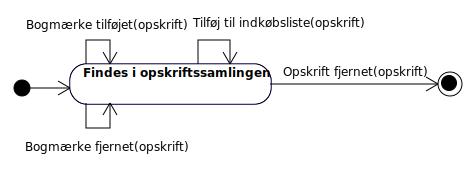
\includegraphics[scale=0.7]{billeder/foodl/opskrift.jpg}
	\capt{Her ses et eksempel på en opskrift, der kan være et resultat på en søgning.}
	\label{fig:foodl-opskrift}
\end{figure}

I toppen af resultatsiden, som er vist på \figref{fig:overblik-resultat}, er der en toolbar, hvorfra brugeren har forskellige muligheder for at manipulere søgningsresultatet. Der er blevet implementeret en toolbar i toppen af siden, der følger brugerens bevægelser mht. at scrolle op og ned. På denne måde behøver brugeren ikke at scrolle helt til toppen for at udføre en handling på søgningsresultatet. 

Figur \ref{fig:foodl-toolbar} præsenterer toolbaren. I venstre side er der en samling af tre knapper, der bruges til at begrænse søgningsresultatet mht. tilberedningstiden. Her er der mulighed for at markere flere af gangen, og default kriteriet er, hvis ingen er markeret, så er alle markeret. Dette betyder, at systemet starter med at vise alle resultater. 
I midten af toolbaren er der et skaleringsværktøj, der kan bruges til at skalere opskrifternes portioner mht. antal personer. Man kan skalere dem ned til en person og op til 10 personer. Vi valgte 10 som maximum, fordi det er relativt let at skalere yderligere, hvis dette er ønsket og det er de færreste gange, man sverer rester for over 10 mennesker.
I højre side af toolbaren er der endnu en samling af tre knapper, men disse benyttes til at sortere opskrifterne. Default er ``relevans''. De to knappesamlinger er forskellige på to måder; hvad de bruges til, og at der kun er mulighed for at markere en knap af gangen ved sorteringsknapperne (højre side) og mulighed for markering af flere af gangen ved afgrænsningsknapperne (venstre side).

\begin{figure}[H]
	\centering
	\includegraphics[scale=0.7]{billeder/foodl/toolbar.jpg}
	\capt{Systemets toolbar, der er direkte under sidehovedet.}
	\label{fig:foodl-toolbar}
\end{figure}

Ud over toolbaren, så viser \figref{fig:foodl-sidebar} en sidebar, hvilket gør det muligt for brugeren at følge med i, hvad der blev søgt på, og den giver brugeren mulighed for at lave endnu en søgning. Man kan herfra slette og/eller tilføje nye råvaretyper til en ny søgning. Denne sidebar følger også med brugeres skærmrulning, da det skal være nemt og hurtigt at lave en ny søgning, hvis dette bliver aktuelt, uanset hvor mange opskrifter, der bliver vist som resultat.

\begin{figure}[H]
	\centering
	\includegraphics[scale=0.7]{billeder/foodl/sidebar.jpg}
	\capt{Systemets sidebar, der vises ved resultatsiden.}
	\label{fig:foodl-sidebar}
\end{figure}

Hvis en bruger vælger at benytte sig af indkøbslisten, så kan denne tilgås via sidehovedet, ved at trykke på ``indkøbsliste''. I sidehovedet kan man også se, hvor mange varer, der allerede er blevet tilføjet til listen.

Hvis brugere opdager en fejl med en af opskrifterne, så er det muligt at rapportere fejl i systemet. På alle opskrifterne er der en trekantet advarsels-knap i nederste højre hjørne, som kan bruges til at rapportere en fejl vedr.\ en opskrift. Figur \ref{fig:foodl-fejlrapportering} viser, hvordan det ser ud, når en bruger trykker på rapporteringsknappen ved en opskrift. Der popper en lille boks op, og baggrunden af siden bliver mørk for at fokusere koncentrationen på oprettelse af fejlrapporten. Her kan man nu specificere, hvad fejlen handler om og evt.\ give en beskrivelse, inden man vælger at indsende fejlen. Beskrivelsesfeltet vises dynamisk i forhold til den valgte fejlkategori.

\begin{figure}[H]
	\centering
	\includegraphics[scale=0.7]{billeder/foodl/fejlrapportering.jpg}
	\capt{Systemets fejlrapportering.}
	\label{fig:foodl-fejlrapportering}
\end{figure}

\subsection{Indkøbsliste}
\label{subsec:brug-indkoebsliste}

Ud over muligheden for at tilføje opskrifternes ingredienser til indkøbslisten, så kan man også tilføje almindelig tekst til, så det er muligt at lave en indkøbsliste, der indeholder andet end ingredienser til madlavningen. Så man kan skrive andre varer på, som man kan købe med fra \fx supermarkedet. Systemets indkøbsliste kan ses i \figref{fig:overblik-indkoebsliste}.

\begin{figure}[H]
	\centering
	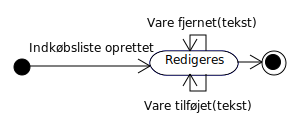
\includegraphics[scale=1]{billeder/foodl/thumbnails/indkoebsliste.png}
	\capt{Denne figur har til formål at give et overblik over systemets indkøbsliste.}
	\label{fig:overblik-indkoebsliste}
\end{figure}

Brugeren har mulighed for at tilføje varer i feltet ``tilføj til indkøbsliste'' og trykke på ``tilføj'' i bunden af siden. Der er mulighed for at slette alle varer fra indkøbslisten, ved at trykke på knappen ``slet alt'' i øverste højre hjørne af indkøbslisten, og ligeledes at slette enkelte varer, ved at trykke på de små gule krydser ud for alle varerne. Derudover er der implementeret en knap, til at udskrive indkøbslisten, som vi naturligvis kalder for ``udskriv''.

Hvis brugeren ikke er logget ind, vil de se i øverste højre hjørne af \figref{fig:overblik-indkoebsliste} (under sidehovedet) en boks, som informerer brugeren om, at man skal være logget ind for at systemet skal være i stand til at gemme indkøbslisten og favoritter. Oprettelse af bruger og indlogning bliver beskrevet nærmere i \secref{subsec:brug-opret}.

\subsection{Favoritliste}
\label{subsec:brug-favoritliste}

Når der bliver tilføjet en opskrift til en brugers favoritliste, så kan denne opskrift findes under ``favoritter'', som kan findes via sidehovedet i toppen af siden. Et eksempel af en kort opskriftsliste under favoritter kan ses på \figref{fig:overblik-favoritter}.

\begin{figure}[H]
	\centering
	\includegraphics[scale=1]{billeder/foodl/thumbnails/favoritter.png}
	\capt{Denne figur har til formål at give et overblik over systemets favoritside.}
	\label{fig:overblik-favoritter}
\end{figure}

En opskrift bliver tilføjet til favoritlisten ved at trykke på den hjerte-formede knap i øverste højre hjørne af en opskrift. Hvis en opskrift ikke er favoriseret, så er det hjerteformede område i knappen gråt. Når den bliver favoriseret, så bliver hjertet rødt, og dette kan ses i \figref{fig:overblik-favoritter}.

Idéen med favoritlisten er at give brugerne mulighed for at gemme opskrifter, de finder interessante og at de gerne vil bogmærke den til næste gang. De er meget nemmere at finde frem, når man kan finde dem under favoritlisten i stedet for at skulle udføre en ny søgning og prøve at finde den samme opskrift igen.

\subsection{Brugeroprettelse}
\label{subsec:brug-opret}

Alle har mulighed for at oprette en bruger på \Foodl{}. Hvis man har en bruger og logger ind på systemet, så kan man kan gemme sin indkøbsliste og listen over favoritter. Det er dog ikke obligatorisk at have en bruger for at kunne bruge systemet, da vi ikke ønsker at binde brugerne til at oprette noget som helst. Man kan bruge hele systemet, om man har en bruger eller ej.

Man opretter en bruger på samme side, hvor man logger ind på systemet. Dette er præsenteret i \figref{fig:overblik-brugeroprettelse}. Man navigerer til denne side ved at klikke på ``log ind / opret bruger'' i højre side af sidehovedet, som også er synlig på samme figur.

\begin{figure}[H]
	\centering
	\includegraphics[scale=0.4]{billeder/foodl/thumbnails/opretbrugeroglogind.png}
	\capt{Denne figur har til formål at give et overblik over systemets brugeroprettelsesside.}
	\label{fig:overblik-brugeroprettelse}
\end{figure}

Man skal bruge sin email og en adgangskode for at lave en bruger. Hvis man allerede har en bruger, så skal man blot logge ind med de rigtige oplysninger.

Når man er logget ind, så ændrer sidehovedet sig en smule. Figur \ref{fig:foodl-loggetind} viser, at der nu er mulighed for at gå ind i en menu, der hedder ``indstillinger'' og at logge ud igen. Man kan også se, at der pludselig er indlæst en liste af favoritter på 10 opskrifter fra tidligere et besøg.

\begin{figure}[H]
	\centering
	\includegraphics[scale=0.4]{billeder/foodl/header-login.png}
	\capt{Det ændrede sidehovede, når brugeren er logget ind.}
	\label{fig:foodl-loggetind}
\end{figure}

Hvis man ønsker at skifte sin adgangskode, så sker det ved at trykke på knappen ``indstillinger'' i sidehovedet.

\subsection{Generelt}
Som de fleste andre hjemmesider, så har vi også en ``om'' og en ``kontakt'' side, som kan tilgås fra nederste venstre hjørne af enhver underside af \Foodl{}. Derudover kan man rapportere en generel fejl ved siden, hvis man støder på sådan en. Figur \ref{fig:foodl-formaliteter} viser disse tre knapper.

\begin{figure}[H]
	\centering
	\includegraphics[scale=0.7]{billeder/foodl/formaliteter.jpg}
	\capt{I nederste venstre hjørne af systemet kan man rapportere en generel fejl, læse mere om systemet og kontakte udviklerne.}
	\label{fig:foodl-formaliteter}
\end{figure}

Under ``om foodl'' kan brugeren kort læse om dette projekt og om udviklerne bag systemet, altså denne gruppe.

\subsection{Designovervejelser}
\label{subsec:designovervejelser}

\todo{DEB!}
